\chapter{Expresión génica: transcripción y traducción}\label{ch:b1:gene-expression}

Un \omterm{def:b1:genomes:gene}{gen} de treinta mil \omterm{thm:b1:nucleic-acids:helix}{pares de bases} se lee en un cuarto de hora hasta
formar una copia de trabajo, se recorta a dos mil letras, se envía fuera del
núcleo y lo traducen veinticinco \omterm{def:b1:gene-expression:ribosome}{ribosomas} a la vez en una \omterm{def:b1:proteins:peptide}{proteína} de
quinientos \omterm{def:b1:proteins:aminoacid}{aminoácidos}: uno cada cuatro segundos, mientras dure la copia. La
\omterm{def:b1:cell-unit-of-life:cell}{célula} gasta en esto más energía que en ninguna otra cosa. Este capítulo
sigue la información desde el \omterm{def:b1:nucleic-acids:chain}{ADN} hasta la \omterm{def:b1:proteins:peptide}{proteína}: la copia de un \omterm{def:b1:genomes:gene}{gen} a
\omterm{def:b1:nucleic-acids:chain}{ARN}, la edición de ese \omterm{def:b1:nucleic-acids:chain}{ARN} en los eucariotas, el código que asigna
\omterm{def:b1:proteins:aminoacid}{aminoácidos} a los tripletes de bases, el \omterm{def:b1:gene-expression:ribosome}{ribosoma} que lo lee, y lo que le
ocurre a una \omterm{def:b1:proteins:peptide}{proteína} una vez fabricada.

\section{Del gen a la proteína}

\begin{proposition}[El flujo de la información]\label{prop:b1:gene-expression:dogma}
\index{expresión génica}\index{transcripción}\index{traducción}
La información genética fluye del \omterm{def:b1:nucleic-acids:chain}{ADN} al \omterm{def:b1:nucleic-acids:chain}{ARN} y del \omterm{def:b1:nucleic-acids:chain}{ARN} a la \omterm{def:b1:proteins:peptide}{proteína}. La
\emph{transcripción} copia una hebra de un \omterm{def:b1:genomes:gene}{gen} a un \omterm{def:b1:nucleic-acids:chain}{ARN} de la misma
secuencia que la otra hebra (con U en lugar de T); la \emph{traducción} lee
el \omterm{def:b1:nucleic-acids:rnas}{ARN mensajero} de tres bases en tres bases y ensambla los \omterm{def:b1:proteins:aminoacid}{aminoácidos}
correspondientes en un \omterm{def:b1:proteins:peptide}{polipéptido}. Todos los pasos usan el apareamiento de
bases: el \omterm{def:b1:nucleic-acids:chain}{ADN} con el \omterm{def:b1:nucleic-acids:chain}{ARN} en la transcripción, y el mensajero con el \omterm{def:b1:gene-expression:trna}{ARN de
transferencia} en la traducción. La secuencia de una \omterm{def:b1:proteins:peptide}{proteína} es, pues, una
transcripción de la secuencia de su \omterm{def:b1:genomes:gene}{gen}, y el cambio de una sola base puede
cambiar un \omterm{def:b1:proteins:aminoacid}{aminoácido}: es el vínculo entre mutación y fenotipo. La
información no fluye de vuelta de la \omterm{def:b1:proteins:peptide}{proteína} al ácido nucleico; el único
paso inverso, el \omterm{def:b1:nucleic-acids:chain}{ARN} copiado a \omterm{def:b1:nucleic-acids:chain}{ADN} por los retrovirus, no toca la \omterm{def:b1:proteins:peptide}{proteína}.
\end{proposition}

\section{La transcripción}

\begin{definition}[ARN polimerasa, promotor, transcripción]\label{def:b1:gene-expression:transcription}
\index{ARN polimerasa}\index{promotor}
La \emph{\omterm{def:b1:nucleic-acids:chain}{ARN} polimerasa} sintetiza \omterm{def:b1:nucleic-acids:chain}{ARN} sobre un molde de \omterm{def:b1:nucleic-acids:chain}{ADN}, de
$5' \to 3'$, a partir de los cuatro ribonucleósidos trifosfato y sin
cebador. Empieza en un \emph{promotor}, una secuencia situada justo aguas
arriba del \omterm{def:b1:genomes:gene}{gen} que la \omterm{def:b1:enzymes:enzyme}{enzima} reconoce y a la que se une; en las bacterias
una subunidad llamada $\sigma$ (\emph{sigma}) se encarga del
reconocimiento, en dos tramos conservados diez y treinta y cinco pares antes
del inicio. La \omterm{def:b1:enzymes:enzyme}{enzima} abre unos quince pares de la hélice formando una
\emph{burbuja de transcripción}, copia la \emph{hebra molde} (leída de
$3' \to 5'$) a un \omterm{def:b1:nucleic-acids:chain}{ARN} de secuencia idéntica a la otra hebra, la
\emph{codificante}, y avanza a unos cincuenta \omterm{def:b1:nucleic-acids:nucleotide}{nucleótidos} por segundo
mientras vuelve a cerrar la hélice tras de sí; el \omterm{def:b1:nucleic-acids:chain}{ARN} se desprende a medida
que se fabrica. Se detiene en un \emph{terminador}: en las bacterias, una
secuencia autocomplementaria cuyo \omterm{def:b1:nucleic-acids:chain}{ARN} se pliega en una horquilla que libera
el transcrito. Muchas polimerasas pueden seguirse unas a otras a lo largo de
un \omterm{def:b1:genomes:gene}{gen}, de modo que puede iniciarse un transcrito cada segundo.
\end{definition}

\begin{omfigure}
\begin{tikzpicture}[font=\footnotesize, >=Stealth, line cap=round]
  % DNA duplex left and right of bubble
  \draw[very thick, omDef] (0,0.5) -- (3.0,0.5); \draw[very thick, omDef!50] (0,-0.5) -- (3.0,-0.5);
  \draw[very thick, omDef] (8.0,0.5) -- (11.5,0.5); \draw[very thick, omDef!50] (8.0,-0.5) -- (11.5,-0.5);
  \foreach \x in {0.4,0.9,...,2.9} { \draw[gray!60] (\x,0.5) -- (\x,-0.5); }
  \foreach \x in {8.4,8.9,...,11.4} { \draw[gray!60] (\x,0.5) -- (\x,-0.5); }
  % bubble: strands separate
  \draw[very thick, omDef] (3.0,0.5) .. controls (4.0,1.3) and (7.0,1.3) .. (8.0,0.5);
  \draw[very thick, omDef!50] (3.0,-0.5) .. controls (4.0,-1.3) and (7.0,-1.3) .. (8.0,-0.5);
  % polymerase
  \draw[thick, omProp!80!black, fill=omProp!25, opacity=0.85] (5.5,0) ellipse (2.3 and 1.7);
  \node[omProp!80!black, anchor=east] at (2.7,1.5) {ARN polimerasa}; \draw[omProp!80!black] (2.75,1.45) -- (3.6,1.0);
  % RNA transcript: paired to template in bubble, then exiting
  \draw[very thick, omThm] (4.0,-0.85) .. controls (5.0,-0.75) .. (6.0,-0.75) .. controls (6.5,-0.4) and (6.3,1.2) .. (5.2,2.3);
  \node[omThm, anchor=south] at (5.1,2.35) {ARN, con el extremo $5'$ emergiendo};
  \draw[thin, omThm] (6.0,-0.8) -- (6.4,-1.95);
  \node[omThm, anchor=north, font=\scriptsize] at (6.4,-2.0) {$3'$: extremo creciente del ARN};
  % labels
  \node[anchor=east, omDef] at (-0.1,0.5) {$5'$ hebra codificante $3'$};
  \node[anchor=east, omDef!70!black] at (-0.1,-0.5) {$3'$ hebra molde $5'$};
  \draw[->, very thick, omProp!80!black] (8.6,1.9) -- (10.2,1.9) node[midway, above] {sentido de la transcripción};
  \node[anchor=north, align=center, gray] at (5.5,-2.55) {el ARN es complementario de la hebra molde e idéntico (con U en lugar de T) a la codificante;\\ hay unos quince pares de bases abiertos a la vez, y la hélice se rehace tras la enzima};
\end{tikzpicture}

{\small La transcripción. La polimerasa abre una burbuja, aparea
ribonucleótidos con la hebra molde y los une de $5' \to 3'$; el \omterm{def:b1:nucleic-acids:chain}{ARN} sale por
un canal a medida que la \omterm{def:b1:enzymes:enzyme}{enzima} avanza.}
\end{omfigure}

\begin{proposition}[Transcripción y maduración del ARN en eucariotas]\label{prop:b1:gene-expression:processing}
\index{corte y empalme}\index{ARN mensajero}\index{caperuza}\index{cola de poli-A}
Los eucariotas tienen tres polimerasas: la I para los \omterm{def:b1:nucleic-acids:rnas}{ARN ribosómicos}
grandes, la II para los \omterm{def:b1:nucleic-acids:rnas}{ARN mensajeros} y la III para los \omterm{def:b1:gene-expression:trna}{ARN de
transferencia} y otros \omterm{def:b1:nucleic-acids:chain}{ARN} pequeños. La polimerasa II no reconoce su \omterm{def:b1:gene-expression:transcription}{promotor}
por sí sola: un conjunto de \emph{factores generales de transcripción} se
ensambla sobre él (en una secuencia TATA situada unos treinta pares aguas
arriba en muchos \omterm{def:b1:genomes:gene}{genes}) y recluta la \omterm{def:b1:enzymes:enzyme}{enzima}, y \omterm{def:b1:proteins:peptide}{proteínas} reguladoras unidas
cerca o lejos modulan la velocidad (\cref{ch:b1:expression-control}). El
transcrito primario se \emph{madura} en el núcleo: se añade una guanina
modificada, la \emph{caperuza}, al extremo $5'$, una cola de unas doscientas
adeninas (\emph{poli-A}) al extremo $3'$, y se retiran los intrones por
\emph{\omterm{prop:b1:gene-expression:processing}{corte y empalme}}: un complejo de \omterm{def:b1:nucleic-acids:chain}{ARN} pequeños y \omterm{def:b1:proteins:peptide}{proteínas}, el
\emph{espliceosoma}, reconoce el GU del inicio de cada \omterm{def:b1:genomes:gene}{intrón} y el AG de su
final, corta y une los exones. Solo entonces se exporta al \omterm{def:b1:eukaryotic-cell:organelle}{citosol} el
mensajero maduro. Muchos \omterm{def:b1:genomes:gene}{genes} se cortan y empalman de más de una manera
(\emph{empalme alternativo}), de modo que un \omterm{def:b1:genomes:gene}{gen} rinde varias \omterm{def:b1:proteins:peptide}{proteínas}; los
veinte mil \omterm{def:b1:genomes:gene}{genes} humanos fabrican quizá cien mil.
\end{proposition}
\begin{proof}[Evidencia]
Sharp y Roberts (1977) hibridaron un \omterm{def:b1:nucleic-acids:rnas}{ARN mensajero} vírico con el \omterm{def:b1:nucleic-acids:chain}{ADN} de su
\omterm{def:b1:genomes:gene}{gen} y observaron los híbridos al \omterm{prop:b1:cell-unit-of-life:microscopes}{microscopio electrónico}: el \omterm{def:b1:nucleic-acids:chain}{ARN} se apareaba
con el \omterm{def:b1:nucleic-acids:chain}{ADN} en varios tramos y, entre ellos, el \omterm{def:b1:nucleic-acids:chain}{ADN} formaba bucles sin
aparear: los intrones, presentes en el \omterm{def:b1:genomes:gene}{gen} y ausentes del mensaje. Los \omterm{def:b1:genomes:gene}{genes}
bacterianos, tratados igual, no daban bucles. El tamaño del transcrito
primario de un \omterm{def:b1:genomes:gene}{gen}, medido en el núcleo, coincide con el \omterm{def:b1:genomes:gene}{gen}; el tamaño del
mensajero citoplásmico coincide solo con los exones.
\end{proof}

\begin{omfigure}
\begin{tikzpicture}[font=\footnotesize, >=Stealth, line cap=round]
  % gene
  \draw[very thick, gray] (0,3.2) -- (11,3.2);
  \fill[omDef!70] (0.6,2.95) rectangle (1.8,3.45); \fill[omDef!70] (4.2,2.95) rectangle (5.4,3.45); \fill[omDef!70] (8.0,2.95) rectangle (9.6,3.45);
  \node[anchor=east] at (-0.1,3.2) {gen};
  \node[anchor=south, font=\scriptsize] at (1.2,3.5) {exón 1}; \node[anchor=south, font=\scriptsize] at (4.8,3.5) {exón 2}; \node[anchor=south, font=\scriptsize] at (8.8,3.5) {exón 3};
  \draw[->, thick] (5.5,2.7) -- (5.5,2.2) node[midway, right] {transcripción};
  % primary transcript
  \draw[very thick, omThm!60] (0.6,1.8) -- (9.6,1.8);
  \fill[omDef!70] (0.6,1.6) rectangle (1.8,2.0); \fill[omDef!70] (4.2,1.6) rectangle (5.4,2.0); \fill[omDef!70] (8.0,1.6) rectangle (9.6,2.0);
  \node[anchor=east] at (-0.1,1.8) {transcrito primario};
  \node[anchor=north, font=\scriptsize] at (3.0,1.55) {intrón 1}; \node[anchor=north, font=\scriptsize] at (6.7,1.55) {intrón 2};
  \draw[->, thick] (5.5,1.2) -- (5.5,0.7) node[pos=0.9, right, align=left] {caperuza, empalme,\\ poliadenilación};
  % mature mRNA
  \fill[omExo!70] (0.2,0.15) circle (0.13); \node[anchor=south, font=\scriptsize] at (0.2,0.3) {caperuza};
  \fill[omDef!70] (0.4,0.0) rectangle (1.6,0.4); \fill[omDef!70] (1.6,0.0) rectangle (2.8,0.4); \fill[omDef!70] (2.8,0.0) rectangle (4.4,0.4);
  \draw[very thick, omExo!70] (4.4,0.2) -- (6.0,0.2); \node[anchor=west, font=\scriptsize] at (6.05,0.2) {cola de poli-A (AAAA\ldots)};
  \node[anchor=east] at (-0.1,0.2) {ARNm maduro};
  \node[anchor=north, align=center, gray] at (5.5,-0.4) {los exones se unen en orden; los intrones, casi todo el transcrito, se degradan en el núcleo};
\end{tikzpicture}

{\small Del \omterm{def:b1:genomes:gene}{gen} al mensajero en un eucariota: se transcribe el \omterm{def:b1:genomes:gene}{gen} entero,
después se recortan los intrones y se unen los exones, se añaden una
caperuza y una \omterm{prop:b1:gene-expression:processing}{cola de poli-A}, y el mensaje maduro sale del núcleo.}
\end{omfigure}

\section{El código genético}

\begin{definition}[El código genético]\label{def:b1:gene-expression:code}
\index{código genético}\index{codón}\index{marco de lectura}
El \emph{código genético} asigna \omterm{def:b1:proteins:aminoacid}{aminoácidos} a los tripletes de bases del
mensajero, los \emph{codones}. De los 64 codones, 61 especifican los veinte
\omterm{def:b1:proteins:aminoacid}{aminoácidos} y tres (UAA, UAG, UGA) son señales de \emph{parada}; AUG
especifica metionina y es además el codón de \emph{inicio}, de modo que todo
\omterm{def:b1:proteins:peptide}{polipéptido} nuevo empieza por metionina. El código es \emph{degenerado} ---
casi todos los \omterm{def:b1:proteins:aminoacid}{aminoácidos} tienen varios codones, que difieren sobre todo en
la tercera posición ---, \emph{no solapado}, se lee sin puntuación en un
\emph{marco de lectura} fijado por el codón de inicio, y es casi
\emph{universal}: el mismo en bacterias, plantas y animales, con variantes
menores en las \omterm{def:b1:eukaryotic-cell:mitochondrion}{mitocondrias}; un \omterm{def:b1:genomes:gene}{gen} humano introducido en una bacteria se
lee correctamente.
\end{definition}

\begin{omfigure}
\begin{center}
\footnotesize
\begin{tabular}{c|cccc|c}
\hline
primera & \multicolumn{4}{c|}{segunda base} & tercera \\
base & U & C & A & G & base \\
\hline
U & Phe Phe Leu Leu & Ser Ser Ser Ser & Tyr Tyr \textbf{parada} \textbf{parada} & Cys Cys \textbf{parada} Trp & U C A G \\
C & Leu Leu Leu Leu & Pro Pro Pro Pro & His His Gln Gln & Arg Arg Arg Arg & U C A G \\
A & Ile Ile Ile \textbf{Met} & Thr Thr Thr Thr & Asn Asn Lys Lys & Ser Ser Arg Arg & U C A G \\
G & Val Val Val Val & Ala Ala Ala Ala & Asp Asp Glu Glu & Gly Gly Gly Gly & U C A G \\
\hline
\end{tabular}
\end{center}

{\small El \omterm{def:b1:gene-expression:code}{código genético}. Cada casilla enumera los cuatro codones con la
primera y la segunda base indicadas y con tercera base U, C, A, G por ese
orden. AUG es metionina y la señal de inicio; UAA, UAG y UGA son paradas. La
tercera base a menudo no importa: el código es degenerado.}
\end{omfigure}

\begin{proposition}[Cómo se descifró el código]\label{prop:b1:gene-expression:nirenberg}
El código es un código de tripletes no solapado, y el significado de cada
\omterm{def:b1:gene-expression:code}{codón} puede determinarse por vía química.
\end{proposition}
\begin{proof}[Evidencia]
Crick y Brenner (1961) produjeron en un \omterm{def:b1:genomes:gene}{gen} de fago mutaciones que añadían o
quitaban una base: un cambio de esos destruía la función del \omterm{def:b1:genomes:gene}{gen}, y dos
también, pero tres inserciones (o tres deleciones) próximas entre sí la
restablecían: el mensaje se lee de tres en tres, desde un punto de partida
fijo, y una inserción desplaza el marco de todo lo que viene después.
Nirenberg y Matthaei (1961) añadieron un \omterm{def:b1:nucleic-acids:chain}{ARN} sintético formado solo por
uracilos a un extracto acelular de \emph{E. coli} con los veinte
\omterm{def:b1:proteins:aminoacid}{aminoácidos}: se fabricó una cadena solo de fenilalanina, luego UUU significa
Phe; otros mensajeros sintéticos, y después la unión de trinucleótidos
sueltos a \omterm{def:b1:gene-expression:ribosome}{ribosomas} con sus \omterm{def:b1:gene-expression:trna}{ARN de transferencia}, asignaron los sesenta y
cuatro en 1966.
\end{proof}

\begin{example}[Leer un mensaje]\label{ex:b1:gene-expression:reading}
El mensajero $5'$-\ldots{}GC\underline{AUG}GCUUUCGGAUAA\ldots{}-$3'$ se lee
desde el AUG: AUG GCU UUC GGA UAA --- Met-Ala-Phe-Gly-parada: un péptido de
cuatro residuos. Elimínese la primera G tras el AUG y el marco se desplaza:
AUG CUU UCG GAU AA\ldots{} --- Met-Leu-Ser-Asp\ldots, una \omterm{def:b1:proteins:peptide}{proteína} distinta
de longitud distinta. Cámbiese UUC por UUU y no cambia nada: ambos son Phe,
una mutación \emph{silenciosa}.
\end{example}

\section{La traducción}

\begin{definition}[El ARN de transferencia y sus sintetasas]\label{def:b1:gene-expression:trna}
\index{ARN de transferencia}\index{anticodón}\index{aminoacil-ARNt sintetasa}
Un \emph{\omterm{def:b1:nucleic-acids:chain}{ARN} de transferencia} (\cref{ch:b1:nucleic-acids}) es el adaptador
entre el \omterm{def:b1:gene-expression:code}{codón} y el \omterm{def:b1:proteins:aminoacid}{aminoácido}: su \emph{anticodón}, tres bases en un bucle,
se aparea de forma antiparalela con un \omterm{def:b1:gene-expression:code}{codón} del mensaje, y su extremo $3'$
lleva el \omterm{def:b1:proteins:aminoacid}{aminoácido} correspondiente. El apareamiento en la tercera posición
del \omterm{def:b1:gene-expression:code}{codón} es laxo (\emph{balanceo}), de modo que unos cuarenta ARNt bastan
para sesenta y un codones. A cada ARNt lo carga su propia
\emph{aminoacil-ARNt sintetasa}, una \omterm{def:b1:enzymes:enzyme}{enzima} que reconoce a la vez el
\omterm{def:b1:proteins:aminoacid}{aminoácido} y el ARNt y los une en dos etapas a costa de un \omterm{def:b1:water-small-molecules:atp}{ATP} (escindido
hasta AMP: dos enlaces ricos en energía), y que corrige el \omterm{def:b1:proteins:aminoacid}{aminoácido}
mientras lo hace. Esas veinte \omterm{def:b1:enzymes:enzyme}{enzimas} son donde el código se aplica
realmente: el \omterm{def:b1:gene-expression:ribosome}{ribosoma} no comprueba qué \omterm{def:b1:proteins:aminoacid}{aminoácido} lleva un ARNt, solo que
su anticodón encaje.
\end{definition}

\begin{definition}[El ribosoma]\label{def:b1:gene-expression:ribosome}
\index{ribosoma}
El \emph{ribosoma} es una partícula de dos subunidades, cada una de \omterm{def:b1:nucleic-acids:rnas}{ARN
ribosómico} y \omterm{def:b1:proteins:peptide}{proteínas} (en las bacterias: una subunidad pequeña 30S y una
grande 50S, juntas 70S, \qty{2.5}{MDa}; los ribosomas eucariotas son
mayores, 80S). La subunidad pequeña se une al mensajero y lo descodifica; la
grande sostiene los ARNt y forma el \omterm{def:b1:proteins:peptide}{enlace peptídico}, y el catalizador es el
propio \omterm{def:b1:nucleic-acids:rnas}{ARN ribosómico}. Tres sitios para ARNt abarcan ambas subunidades: el A
(aminoacil, donde entra el siguiente ARNt cargado), el P (peptidil, que
sostiene la cadena en crecimiento) y el E (salida).
\end{definition}

\begin{omfigure}
\begin{tikzpicture}
  \node[anchor=south west, inner sep=0] (img) at (0,0)
    {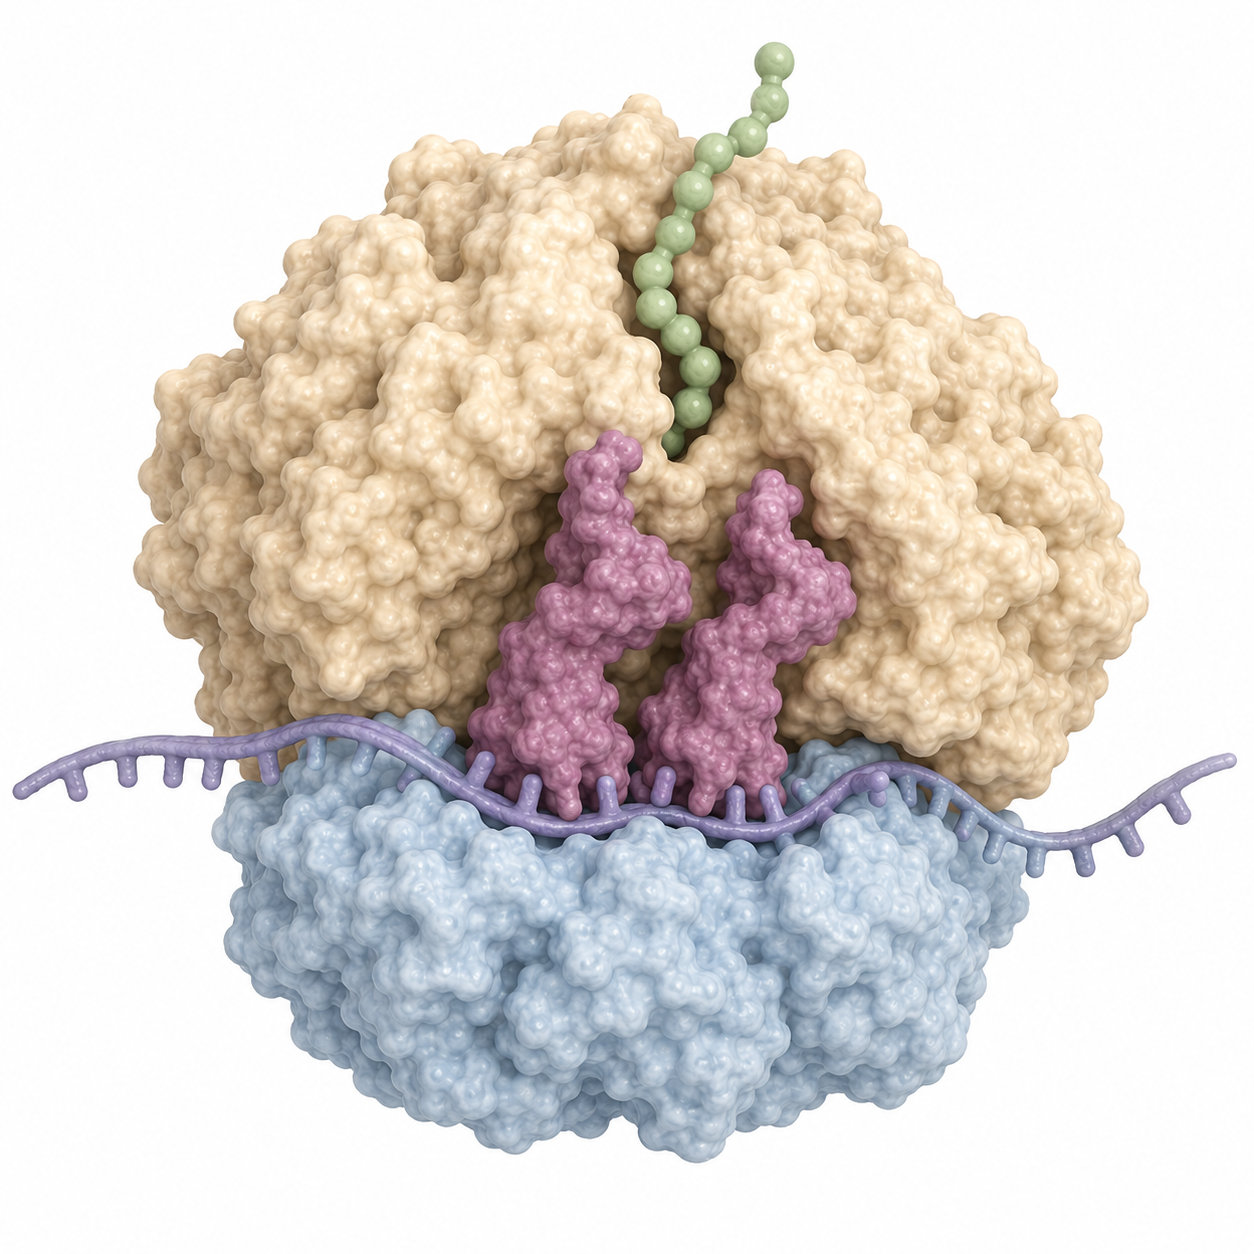
\includegraphics[width=0.46\linewidth]{images/book3/ai/fig-ribosome-3d.png}};
  \begin{scope}[x={(img.south east)}, y={(img.north west)},
      every node/.style={font=\small}]
    \draw[omDef, thick] (0.30,0.72) -- (0.30,1.08) node[above] {subunidad grande: aquí se forma el enlace peptídico};
    \draw[omDef, thick] (0.50,0.15) -- (0.50,-0.08) node[below] {subunidad pequeña: descodifica el mensaje};
    \draw[omDef, thick] (0.47,0.52) -- (-0.03,0.44) node[left, align=right] {ARNt en los\\ sitios P y A};
    \draw[omDef, thick] (0.92,0.36) -- (1.03,0.26) node[right] {ARNm};
    \draw[omDef, thick] (0.57,0.88) -- (1.03,0.90) node[right, align=left] {polipéptido que sale\\ por el túnel de salida};
  \end{scope}
\end{tikzpicture}

{\small El \omterm{def:b1:gene-expression:ribosome}{ribosoma}: dos subunidades acopladas sobre el mensajero, dos \omterm{def:b1:gene-expression:trna}{ARN
de transferencia} en la hendidura y la cadena en crecimiento saliendo por un
túnel de la subunidad grande.}
\end{omfigure}

\begin{proposition}[El ciclo de elongación]\label{prop:b1:gene-expression:elongation}
La traducción empieza cuando la subunidad pequeña encuentra el \omterm{def:b1:gene-expression:code}{codón} de
inicio --- en las bacterias apareando una secuencia del \omterm{def:b1:nucleic-acids:rnas}{ARN ribosómico} con
un sitio situado justo aguas arriba del AUG, y en los eucariotas uniéndose a
la caperuza y rastreando hasta el primer AUG --- y el ARNt iniciador
(metionina) se aloja en el sitio P; después se une la subunidad grande. Cada
vuelta de \emph{elongación} añade un residuo: un factor de elongación
entrega y comprueba un ARNt cargado cuyo \omterm{def:b1:gene-expression:trna}{anticodón} encaje con el \omterm{def:b1:gene-expression:code}{codón} del
sitio A (un GTP); el \omterm{def:b1:nucleic-acids:rnas}{ARN ribosómico} de la subunidad grande transfiere la
cadena en crecimiento desde el ARNt del sitio P al \omterm{def:b1:proteins:aminoacid}{aminoácido} del ARNt del
sitio A y forma el \omterm{def:b1:proteins:peptide}{enlace peptídico}; el \omterm{def:b1:gene-expression:ribosome}{ribosoma} avanza un \omterm{def:b1:gene-expression:code}{codón} (un segundo
GTP), con lo que los ARNt pasan a P y a E, y el vacío se marcha. En un \omterm{def:b1:gene-expression:code}{codón}
de parada, un \emph{factor de liberación} entra en el sitio A y la cadena se
libera por \omterm{prop:b1:water-small-molecules:families}{hidrólisis}. Los \omterm{def:b1:gene-expression:ribosome}{ribosomas} bacterianos añaden de quince a veinte
residuos por segundo y los eucariotas de dos a cinco; varios \omterm{def:b1:gene-expression:ribosome}{ribosomas} leen
un mismo mensaje a la vez y forman un \emph{polisoma}.
\end{proposition}

\begin{omfigure}
\begin{tikzpicture}[font=\footnotesize, >=Stealth, line cap=round,
  rib/.style={draw, thick, rounded corners=8pt, fill=omDef!12, minimum width=30mm, minimum height=14mm},
  trna/.style={draw, thick, fill=omProp!30, minimum width=6mm, minimum height=9mm, inner sep=1pt, font=\scriptsize}]
  \foreach \i/\title in {0/{1. entra un ARNt cargado en el sitio A}, 1/{2. enlace peptídico: la cadena pasa al ARNt del sitio A}, 2/{3. translocación: el ribosoma avanza un codón}} {
    \begin{scope}[xshift=\i*4.5cm]
      \node[rib] (r) at (0,0) {};
      \draw[very thick, omThm] (-2.0,-0.9) -- (2.0,-0.9);
      \node[font=\scriptsize] at (-0.45,-0.55) {P}; \node[font=\scriptsize] at (0.45,-0.55) {A};
      \node[anchor=north, align=center, font=\scriptsize, text width=40mm] at (0,-1.75) {\title};
    \end{scope}
  }
  % state 1: P holds chain, A receives new tRNA
  \node[trna] at (-0.45,0.05) {}; \draw[very thick, omExo!70!black] (-0.45,0.5) -- (-0.45,1.4); \foreach \y in {0.6,0.85,1.1,1.35} { \fill[omExo!70!black] (-0.45,\y) circle (0.09); }
  \node[trna] at (0.45,0.05) {}; \fill[omExo!70!black] (0.45,0.6) circle (0.09);
  \draw[->, thick, omProp!80!black] (1.6,1.3) -- (0.75,0.7); \node[font=\scriptsize, anchor=west] at (1.4,1.45) {GTP};
  % state 2: chain transferred
  \node[trna] at (4.05,0.05) {}; \node[trna] at (4.95,0.05) {}; \draw[very thick, omExo!70!black] (4.95,0.5) -- (4.95,1.65); \foreach \y in {0.6,0.85,1.1,1.35,1.6} { \fill[omExo!70!black] (4.95,\y) circle (0.09); }
  % state 3: translocated: chain on P, empty tRNA leaving at E, A free
  \node[trna, fill=gray!20] at (7.6,0.05) {}; \node[trna] at (8.55,0.05) {}; \draw[very thick, omExo!70!black] (8.55,0.5) -- (8.55,1.65); \foreach \y in {0.6,0.85,1.1,1.35,1.6} { \fill[omExo!70!black] (8.55,\y) circle (0.09); }
  \draw[->, thick, gray] (7.6,-0.4) -- (7.0,-1.0); \node[font=\scriptsize, gray, anchor=east] at (7.05,-0.4) {E};
  \draw[->, thick, omProp!80!black] (10.7,0.3) -- (10.7,-0.3); \node[font=\scriptsize, anchor=west] at (10.8,0.3) {GTP};
  \draw[->, thick, omThm] (9.4,-1.3) -- (10.4,-1.3) node[right, font=\scriptsize, omThm] {el ARNm se desplaza};
\end{tikzpicture}

{\small Una vuelta de elongación. Se admite un ARNt cargado en el sitio A
cuando su \omterm{def:b1:gene-expression:trna}{anticodón} encaja; el \omterm{def:b1:nucleic-acids:rnas}{ARN ribosómico} une la cadena a su \omterm{def:b1:proteins:aminoacid}{aminoácido};
el \omterm{def:b1:gene-expression:ribosome}{ribosoma} avanza un \omterm{def:b1:gene-expression:code}{codón} y el ARNt vacío se marcha. Dos GTP por residuo,
más los dos enlaces ricos en energía gastados en cargar el ARNt.}
\end{omfigure}

\begin{omfigure}
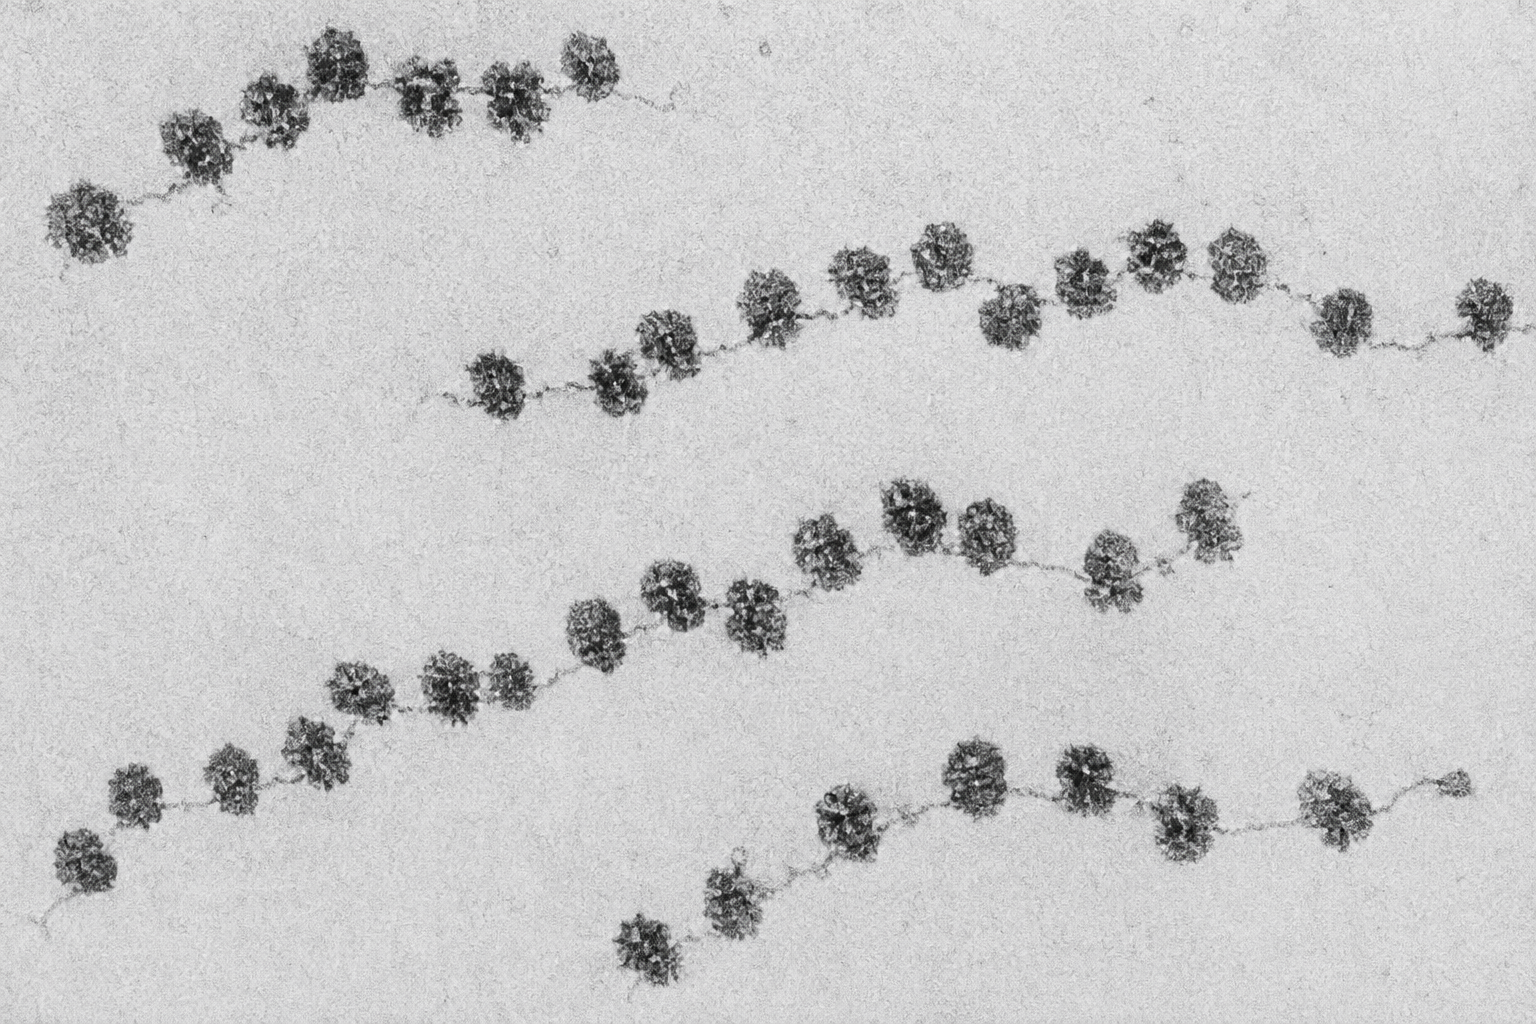
\includegraphics[width=0.5\linewidth]{images/book3/ai/b3-19-polysome-tem.png}

{\small Polisomas al \omterm{prop:b1:cell-unit-of-life:microscopes}{microscopio electrónico}: \omterm{def:b1:gene-expression:ribosome}{ribosomas} ensartados a lo
largo de un mensajero, cada uno fabricando su propia copia de la \omterm{def:b1:proteins:peptide}{proteína}.}
\end{omfigure}

\begin{method}[Cálculo de la síntesis de una proteína]\label{met:b1:gene-expression:reckon}
\begin{enumerate}
  \item Longitud: una \omterm{def:b1:proteins:peptide}{proteína} de $n$ residuos necesita una secuencia
        codificante de $3n + 3$ \omterm{def:b1:nucleic-acids:nucleotide}{nucleótidos} (incluido el \omterm{def:b1:gene-expression:code}{codón} de parada),
        dentro de un mensajero más largo por sus extremos no traducidos y,
        en el \omterm{def:b1:genomes:gene}{gen}, por sus intrones.
  \item Tiempo: divídase $n$ por la velocidad de elongación (de
        \qtyrange{15}{20}{} por segundo en las bacterias y de
        \qtyrange{2}{5}{} en los eucariotas); el mensaje lo lee un \omterm{def:b1:gene-expression:ribosome}{ribosoma}
        cada \qtyrange{80}{100}{} \omterm{def:b1:nucleic-acids:nucleotide}{nucleótidos}, así que la producción por
        mensaje es una cadena cada (separación / velocidad) segundos.
  \item Energía: cuatro enlaces fosfato ricos en energía por residuo (dos
        para cargar el ARNt y dos GTP en el \omterm{def:b1:gene-expression:ribosome}{ribosoma}), más la transcripción
        del mensaje a dos por \omterm{def:b1:nucleic-acids:nucleotide}{nucleótido}, repartida entre todas las cadenas
        que rinde ese mensaje.
  \item Fidelidad: alrededor de un \omterm{def:b1:proteins:aminoacid}{aminoácido} equivocado por cada $10^4$
        codones; una \omterm{def:b1:proteins:peptide}{proteína} de \qty{500}{} residuos está mal en algún
        punto en una copia de cada veinte, lo que se tolera porque las
        \omterm{def:b1:proteins:peptide}{proteínas} son reemplazables y los errores no se heredan.
\end{enumerate}
\end{method}

\section{Después de la traducción}

\begin{proposition}[Qué le ocurre a un polipéptido nuevo]\label{prop:b1:gene-expression:after}
\index{péptido señal}\index{modificación postraduccional}
La cadena se pliega a medida que emerge, con la ayuda de las \omterm{prop:b1:proteins:denaturation}{chaperonas}
(\cref{ch:b1:proteins}). Su destino está escrito en su secuencia: un
\emph{\omterm{prop:b1:gene-expression:after}{péptido señal}} del extremo N se une a una \emph{partícula de
reconocimiento de la señal} que detiene la traducción, acopla el \omterm{def:b1:gene-expression:ribosome}{ribosoma} al
\omterm{def:b1:eukaryotic-cell:endomembrane}{retículo endoplasmático} y enhebra la cadena en su luz
(\cref{ch:b1:eukaryotic-cell}); otras secuencias dirigen \omterm{def:b1:proteins:peptide}{proteínas} a las
\omterm{def:b1:eukaryotic-cell:mitochondrion}{mitocondrias}, los \omterm{def:b1:eukaryotic-cell:plastid}{cloroplastos}, el núcleo o los \omterm{def:b1:eukaryotic-cell:peroxisome}{peroxisomas} tras la
síntesis; y una \omterm{def:b1:proteins:peptide}{proteína} sin señal se queda en el \omterm{def:b1:eukaryotic-cell:organelle}{citosol}. Muchas \omterm{def:b1:proteins:peptide}{proteínas}
se \emph{modifican}: se retira la metionina inicial, se añaden azúcares en
el RE y en el \omterm{def:b1:eukaryotic-cell:endomembrane}{Golgi}, las quinasas y las fosfatasas añaden y retiran
fosfatos, se unen \omterm{def:b1:lipids:fattyacid}{lípidos}, se cortan trozos (la insulina se fabrica como una
sola cadena y se corta en dos; los zimógenos se cortan para activarse). Y
toda \omterm{def:b1:proteins:peptide}{proteína} acaba \emph{degradada}: se marca con una \omterm{def:b1:proteins:peptide}{proteína} pequeña, la
\emph{ubiquitina}, y el \emph{proteasoma} la despliega y la digiere, tras
una vida de minutos (las \omterm{def:b1:proteins:peptide}{proteínas} reguladoras) a meses (la hemoglobina), de
modo que las \omterm{def:b1:proteins:peptide}{proteínas} presentes son las que la \omterm{def:b1:cell-unit-of-life:cell}{célula} está fabricando en
ese momento.
\end{proposition}

\begin{example}[Las cifras de una célula]\label{ex:b1:gene-expression:numbers}
Una \emph{E. coli} en crecimiento contiene unos \num{20000} \omterm{def:b1:gene-expression:ribosome}{ribosomas}, cada
uno de los cuales añade veinte residuos por segundo: $\num{4e5}$ residuos
por segundo, un millón de \omterm{def:b1:proteins:peptide}{proteínas} de \qty{300}{} residuos en una hora, es
decir, su propio contenido, que es lo que exige duplicarse cada hora. La
mitad de su energía va a la síntesis de \omterm{def:b1:proteins:peptide}{proteínas}. Una \omterm{def:b1:cell-unit-of-life:cell}{célula} hepática
contiene diez millones de \omterm{def:b1:gene-expression:ribosome}{ribosomas} y fabrica \omterm{def:b1:proteins:peptide}{proteínas} para semanas de uso
y no para dividirse; una \omterm{def:b1:cell-unit-of-life:cell}{célula} plasmática, que secreta anticuerpos, dedica
casi todos a una sola \omterm{def:b1:proteins:peptide}{proteína} y vierte dos mil moléculas por segundo.
\end{example}

\section{Ejercicios}

\begin{exercise}[$\star$]\label{exo:b1:gene-expression:1}
Dese el \omterm{def:b1:nucleic-acids:chain}{ARN} transcrito a partir de la hebra molde $3'$-TACGGATTC-$5'$, y la
hebra codificante.
\end{exercise}

\begin{exercise}[$\star$]\label{exo:b1:gene-expression:2}
Enumérense las tres modificaciones que sufre un transcrito primario
eucariota antes de salir del núcleo.
\end{exercise}

\begin{exercise}[$\star$]\label{exo:b1:gene-expression:3}
Con la tabla del código, tradúzcase $5'$-AUGCCGAAAGUUUGA-$3'$.
\end{exercise}

\begin{exercise}[$\star$]\label{exo:b1:gene-expression:4}
Nómbrense los tres sitios para ARNt del \omterm{def:b1:gene-expression:ribosome}{ribosoma} y qué ocurre en cada uno.
\end{exercise}

\begin{exercise}[$\star\star$]\label{exo:b1:gene-expression:5}
Un mensajero de \qty{2400}{} \omterm{def:b1:nucleic-acids:nucleotide}{nucleótidos} tiene \qty{150}{} de región no
traducida $5'$ y \qty{450}{} de región no traducida $3'$ y poli-A. ¿Cuántos
residuos tiene la \omterm{def:b1:proteins:peptide}{proteína}? ¿Cuánto tarda un \omterm{def:b1:gene-expression:ribosome}{ribosoma} en fabricarla a cuatro
residuos por segundo, y cuántos \omterm{def:b1:gene-expression:ribosome}{ribosomas} pueden leer el mensaje a la vez, a
uno por cada \qty{90}{} \omterm{def:b1:nucleic-acids:nucleotide}{nucleótidos}?
\end{exercise}

\begin{exercise}[$\star\star$]\label{exo:b1:gene-expression:6}
Explíquese por qué tres inserciones restablecen el \omterm{def:b1:gene-expression:code}{marco de lectura} de un
\omterm{def:b1:genomes:gene}{gen} y una o dos no, y qué aspecto tiene la \omterm{def:b1:proteins:peptide}{proteína} fabricada a partir de la
inserción triple.
\end{exercise}

\begin{exercise}[$\star\star$]\label{exo:b1:gene-expression:7}
Una mutación cambia el \omterm{def:b1:gene-expression:code}{codón} CAG por UAG en mitad de un \omterm{def:b1:genomes:gene}{gen} de \qty{300}{}
codones; otra cambia CAG por CAA; y una tercera lo cambia por CGG. Dese el
efecto de cada una sobre la \omterm{def:b1:proteins:peptide}{proteína}.
\end{exercise}

\begin{exercise}[$\star\star$]\label{exo:b1:gene-expression:8}
Explíquese por qué la fidelidad de la traducción descansa en las
\omterm{def:b1:gene-expression:trna}{aminoacil-ARNt sintetasas} y no en el \omterm{def:b1:gene-expression:ribosome}{ribosoma}, y descríbase un experimento
que lo demostrara (una cisteína unida a su ARNt se convierte químicamente en
alanina; ¿dónde acaba la alanina?).
\end{exercise}

\begin{exercise}[$\star\star$]\label{exo:b1:gene-expression:9}
Calcúlense el coste energético, en enlaces ricos en energía, de una \omterm{def:b1:proteins:peptide}{proteína}
de \qty{400}{} residuos, y la fracción de ese coste que corresponde al
\omterm{def:b1:gene-expression:ribosome}{ribosoma}.
\end{exercise}

\begin{exercise}[$\star\star\star$]\label{exo:b1:gene-expression:10}
En las bacterias los \omterm{def:b1:gene-expression:ribosome}{ribosomas} empiezan a traducir un mensaje mientras
todavía se está transcribiendo; en los eucariotas no pueden. Explíquese por
qué (dos razones), y qué hace posible esa diferencia en los eucariotas.
\end{exercise}

\begin{exercise}[$\star\star\star$]\label{exo:b1:gene-expression:11}
Un \omterm{def:b1:genomes:gene}{gen} de cinco exones puede empalmarse incluyendo o saltándose el \omterm{def:b1:genomes:gene}{exón} 3
(\qty{90}{} \omterm{def:b1:nucleic-acids:nucleotide}{nucleótidos}) y el \omterm{def:b1:genomes:gene}{exón} 4 (\qty{100}{} \omterm{def:b1:nucleic-acids:nucleotide}{nucleótidos}). Enumérense
los mensajeros posibles y dígase cuáles conservan el \omterm{def:b1:gene-expression:code}{marco de lectura} del
\omterm{def:b1:genomes:gene}{exón} 5. ¿Qué muestra esto sobre el empalme alternativo?
\end{exercise}

\begin{exercise}[$\star\star\star$]\label{exo:b1:gene-expression:12}
``El código es un accidente congelado: arbitrario, pero demasiado costoso de
cambiar.'' Discútase en un párrafo: qué parece arbitrario en el código, qué
parece optimizado (la tercera posición, codones parecidos para \omterm{def:b1:proteins:aminoacid}{aminoácidos}
parecidos) y por qué una mutación que cambie la especificidad de una
sintetasa es casi siempre letal.
\end{exercise}

\section{Problema: de un gen a una proteína}

\begin{problem}[{Problema de fin de semana --- un gen de treinta kilobases
seguido hasta una proteína de quinientos residuos: transcripción
cronometrada, empalme pesado, ribosomas contados, energía y errores
calculados, hasta llegar al coste en ATP de una proteína}]
\label{pb:b1:gene-expression:1}
Un \omterm{def:b1:genomes:gene}{gen} humano abarca \qty{30}{kb} con ocho exones que suman \qty{2000}{}
\omterm{def:b1:nucleic-acids:nucleotide}{nucleótidos} de mensajero maduro, de los cuales \qty{1503}{} codifican (500
residuos más la parada). La polimerasa II transcribe a \qty{30}{}
\omterm{def:b1:nucleic-acids:nucleotide}{nucleótidos} por segundo; los \omterm{def:b1:gene-expression:ribosome}{ribosomas} alargan a \qty{4}{} residuos por
segundo y se espacian uno cada \qty{80}{} \omterm{def:b1:nucleic-acids:nucleotide}{nucleótidos}; la vida media del
mensajero es de \qty{2}{h}. Costes: dos enlaces ricos en energía por
\omterm{def:b1:nucleic-acids:nucleotide}{nucleótido} transcrito y cuatro por residuo traducido; tómese un enlace rico
en energía como un \omterm{def:b1:water-small-molecules:atp}{ATP}. Tasas de error: $10^{-5}$ por \omterm{def:b1:nucleic-acids:nucleotide}{nucleótido} transcrito
y $10^{-4}$ por \omterm{def:b1:gene-expression:code}{codón} traducido.

\medskip
\noindent\textbf{Parte I --- Transcripción y empalme.}
\begin{enumerate}
  \item ¿Cuánto tarda una polimerasa en transcribir el \omterm{def:b1:genomes:gene}{gen}?
  \item ¿Qué fracción del transcrito primario retira el empalme?
  \item ¿Cuántos \omterm{def:b1:nucleic-acids:nucleotide}{nucleótidos} se transcriben por cada \omterm{def:b1:nucleic-acids:nucleotide}{nucleótido} de
        mensajero maduro?
  \item Calcúlese el \omterm{def:b1:water-small-molecules:atp}{ATP} gastado en transcribir un transcrito primario.
  \item Si una polimerasa arranca cada \qty{10}{s}, ¿cuántas polimerasas
        hay a la vez sobre el \omterm{def:b1:genomes:gene}{gen}, y cuántos mensajeros produce el \omterm{def:b1:genomes:gene}{gen} por
        hora?
  \item Calcúlense el número de intrones y su longitud media.
  \item El espliceosoma retira cada \omterm{def:b1:genomes:gene}{intrón} en aproximadamente un minuto, en
        paralelo. ¿Qué fija el tiempo desde el \omterm{def:b1:genomes:gene}{gen} hasta el mensajero, el
        empalme o la transcripción?
  \item Calcúlense la longitud física del \omterm{def:b1:genomes:gene}{gen} y la del mensajero maduro
        (\qty{0.34}{nm} por \omterm{def:b1:nucleic-acids:nucleotide}{nucleótido}).
\end{enumerate}

\medskip
\noindent\textbf{Parte II --- Traducción.}
\begin{enumerate}[resume]
  \item ¿Cuánto tarda un \omterm{def:b1:gene-expression:ribosome}{ribosoma} en traducir la \omterm{def:b1:proteins:peptide}{proteína}?
  \item ¿Cuántos \omterm{def:b1:gene-expression:ribosome}{ribosomas} leen a la vez un mensajero?
  \item ¿Cuántas moléculas de \omterm{def:b1:proteins:peptide}{proteína} rinde un mensajero por hora?
  \item A lo largo de su vida media de \qty{2}{h}, ¿cuántas rinde en total
        (un mensaje de vida media $t_{1/2}$ rinde, de promedio,
        $t_{1/2}/\ln 2$ horas de producción plena)?
  \item Calcúlese el \omterm{def:b1:water-small-molecules:atp}{ATP} gastado en traducir una \omterm{def:b1:proteins:peptide}{proteína}.
  \item Calcúlese el \omterm{def:b1:water-small-molecules:atp}{ATP} gastado en la transcripción por \omterm{def:b1:proteins:peptide}{proteína},
        repartiendo el coste del transcrito entre las \omterm{def:b1:proteins:peptide}{proteínas} de la
        pregunta 12.
  \item Calcúlense el coste total de una \omterm{def:b1:proteins:peptide}{proteína} y la fracción debida a la
        traducción.
\end{enumerate}

\medskip
\noindent\textbf{Parte III --- Errores.}
\begin{enumerate}[resume]
  \item Calcúlese la probabilidad de que un mensajero dado lleve al menos
        un error de transcripción en sus \qty{1503}{} \omterm{def:b1:nucleic-acids:nucleotide}{nucleótidos}
        codificantes.
  \item Calcúlese la probabilidad de que una molécula dada de \omterm{def:b1:proteins:peptide}{proteína}
        lleve al menos un error de traducción.
  \item Alrededor de una cuarta parte de los cambios de \omterm{def:b1:nucleic-acids:nucleotide}{nucleótido} son
        silenciosos y un tercio de las sustituciones de \omterm{def:b1:proteins:aminoacid}{aminoácido} son
        inocuas. ¿Qué fracción de las moléculas de \omterm{def:b1:proteins:peptide}{proteína} fabricadas es
        defectuosa?
  \item Un mensajero defectuoso rinde \omterm{def:b1:proteins:peptide}{proteínas} defectuosas durante dos
        horas; una \omterm{def:b1:proteins:peptide}{proteína} defectuosa es una sola molécula. Explíquese por
        qué la \omterm{def:b1:cell-unit-of-life:cell}{célula} puede permitirse una tasa de error de traducción diez
        veces la de transcripción, y ambas muy por encima de la de
        replicación.
\end{enumerate}

\medskip
\noindent\textbf{Parte IV --- El presupuesto de la \omterm{def:b1:cell-unit-of-life:cell}{célula}.}
La \omterm{def:b1:cell-unit-of-life:cell}{célula} fabrica \num{3000} copias de esta \omterm{def:b1:proteins:peptide}{proteína} por hora y, en total,
\num{3e9} residuos de \omterm{def:b1:proteins:peptide}{proteína} al día.
\begin{enumerate}[resume]
  \item ¿Cuántos mensajeros de este \omterm{def:b1:genomes:gene}{gen} deben estar presentes a la vez
        (rindiendo cada uno la cantidad de la pregunta 11)?
  \item ¿Cuántos \omterm{def:b1:gene-expression:ribosome}{ribosomas} ocupa esta \omterm{def:b1:proteins:peptide}{proteína}?
  \item Calcúlense el \omterm{def:b1:water-small-molecules:atp}{ATP} diario que la \omterm{def:b1:cell-unit-of-life:cell}{célula} gasta en toda su síntesis de
        \omterm{def:b1:proteins:peptide}{proteínas} (cuatro por residuo) y, a \qty{50}{kJ/mol}, la potencia
        en vatios para una \omterm{def:b1:cell-unit-of-life:cell}{célula} de \qty{2000}{\micro m^3}.
  \item Compárese con la potencia total de la \omterm{def:b1:cell-unit-of-life:cell}{célula} si consume
        \qty{1e9}{} \omterm{def:b1:water-small-molecules:atp}{ATP} por segundo.
  \item Un fármaco bloquea el espliceosoma. Predígase su efecto sobre esta
        \omterm{def:b1:proteins:peptide}{proteína} y sobre una \omterm{def:b1:proteins:peptide}{proteína} bacteriana.
  \item Enúnciese el resultado: el coste en \omterm{def:b1:water-small-molecules:atp}{ATP} de una molécula de la
        \omterm{def:b1:proteins:peptide}{proteína}, repartido entre traducción y transcripción, y el tiempo
        desde el inicio de la transcripción hasta la primera \omterm{def:b1:proteins:peptide}{proteína}
        terminada.
\end{enumerate}
\end{problem}
